\subsection{Algoritmo} \label{sec:algo}
Pela descrição do problema, para definir os tutores de cada aluno o sistema
utiliza uma Árvore Binária de Busca (ABB), em que o pai do aluno na árvore é seu
tutor. Entretanto, o custo da inserção seria proibitivo se utilizássemos a mesma
estrutura para encontrar os tutores, que no pior caso, seria uma árvore
binária degenerada com complexidade de inserção e busca $O(n)$.

Observa-se que a ABB define uma sequência de matrículas
relacionada a um determinado percurso e a estrutura da árvore. Nossa solução (algoritmo~\ref{alg:parent}) propõe 
modelar a mesma sequência, entretanto utilizando uma árvore binária balanceada auxiliar
para calcular os pais e altura dos alunos em relação a ABB original.

Como a árvore binária balanceada auxiliar foi escolhido utilizar a \textit{Splay Tree}, que não tem garantia de uma árvore com altura $O(\lg n)$, mas a complexidade amortizada de $O(m \lg n)$ para uma sequência de $m$ operações. Para guardar os pais e alturas dos alunos na ABB foi escolhido a \textit{Hash Table} com tratamento de colisão por encadeamento.

\begin{algorithm}[ht]
  \small
  \caption{Calcula o pai (tutor) de cada matrícula, modelando a sequência \textit{inorder} de uma Árvore Binária de Busca (ABB) utilizando uma árvore binária balanceada.}
  \label{alg:parent}
  \begin{algorithmic}[1]
    \Require $mat[N]$ vetor de matrículas de tamanho $N$; $parent$ tabela \textit{hash}.
    \Procedure{Parents}{$mat[N], parent$}% \Comment{Vetor de matrículas de tamanho $N$.}
    % \State $keys[N] \gets 0$\Comment{Vetor de chaves com tamanho $N$.}
    \State $order \gets$ \Call{SplayTree}{ }
    % \State $parent \gets$ \Call{HashTable}{N}
    \State $level \gets$ \Call{HashTable}{N}

    \Statex
    \For{$i \gets 0, N-1$}
    % \State $keys[i] \gets mat[i]$

    \If{$order \neq \emptyset$}
    \State \Call{ParentsInner}{$mat$, $parent$, $order$, $level$}
    \EndIf \Comment{$order \neq \emptyset$}
    \Statex
    
    \State \Call{Insert}{$order, mat[i]$}
    % \State $i \gets i + 1$
    
    \EndFor
    \EndProcedure
  \end{algorithmic}
\end{algorithm}

\begin{algorithm}[ht]
  \small
  \caption{Procedimento interno de \textsc{Parents}.}
  \label{alg:parent_inner}
  \begin{algorithmic}[1]
    \Require $mat[N]$ vetor de matrículas de tamanho $N$; $parent$ tabela \textit{hash}.
    \Procedure{ParentsInner}{$mat$, $parent$, $order$, $level$}
    \State $upper \gets$ \Call{LowerBound}{$order, mat[i]$}
    \Statex
    \If{$upper$ not found}
    % \State // Matrículas são menores que $mat[i]$. Sequência ord.: $\ldots
    % W X$
    % \Statex
    \State $w \gets$ \Call{Max}{$order$} \Comment{Maior elemento de $order$.}
    \State $l \gets$ \Call{LookUp}{$level, w+1$} \Comment{$l = level[w+1]$}
    \State \Call{Insert}{$parent, mat[i], w$} \Comment{$parent[mat[i]] = w$}
    \State \Call{Insert}{$level, mat[i], l$}
    \Statex
    \ElsIf{$upper = $ \Call{Min}{$order$}} \Comment{Menor elemento de $order$}
    % \State // Matrículas são maiores que $x$. Sequência ord.: $X W
    % \ldots$
    % \State $w \gets$ \Call{Min}{$order$}
    \State $l \gets$ \Call{LookUp}{$level, upper+1$}
    \State \Call{Insert}{$parent, mat[i],upper$}
    \State \Call{Insert}{$level, mat[i],l$}
    \Statex
    \Else
    \State $lower \gets$ \Call{Previous}{$order, upper$} \Comment{Elemento anterior em $order$}
    \Statex
    % \State // $lower$ e $upper$ estão no meio. Sequência ord.: $\ldots~ L ~
    % X ~ U ~\ldots$
    % \Statex
    % \State // $upper$ é o pai? $upper$ está na subárvore de $lower$?
    \If{\Call{LookUp}{$level, upper$} $>$ \Call{LookUp}{$level, lower$}}
    \State $l \gets$ \Call{LookUp}{$level, upper$}
    \State \Call{Insert}{$parent, mat[i], upper$}
    \State \Call{Insert}{$level, mat[i], l+1$}
    \Statex
    \Else
    % \State // $lower$ é o pai? $lower$ está na subárvore de $upper$?
    \State $l \gets$ \Call{LookUp}{$level, lower$}
    \State \Call{Insert}{$parent, mat[i], lower$}
    \State \Call{Insert}{$level, mat[i], l+1$}
    \EndIf
    \EndIf \Comment{$upper$ not found}
    
    \EndProcedure
  \end{algorithmic}
\end{algorithm}

O algoritmo recebe uma lista de matrículas ($mat$) e uma tabela ($parent$) associando alunos e
tutores vazia. Inicialmente definimos uma \textit{Splay Tree} ($order$), aonde
serão feitas as inserções das matrículas, e outra tabela ($level$) associando a matrícula à
altura na árvore original, linhas 2 e 3. Após a inicialização, percorremos todos
os alunos (linha 4), simulando o percurso original (procedimento \textsc{ParentsInner}) e finalmente
inserimos na árvore balanceada (linha 29).

Dentro do procedimento \textsc{ParentsInner} queremos
encontrar qual posição da sequência a matrícula $i$ ($mat[i]$) encaixará,
para isso procuramos (linha 2) pela menor matrícula ($upper$) tal que seja maior
ou igual à matrícula $i$ ($mat[i]$) na árvore $order$. Caso a matrícula ($upper$) não
exista, podemos concluir que nossa sequência terá o seguinte formato após inserção: $(\ldots,
w,mat[i])$, ou seja $mat[i]$ é maior que todas as matrículas na ABB e filho de $w$. Assim obtemos o maior elemento da sequência ($w$ linha
4) e a altura ($l$) na qual $mat[i]$ seria inserido na árvore (linha 5),
finalmente atualizamos as tabelas de pais e alturas com os novos dados de $mat[i]$
(linhas 6--7). Caso a matrícula exista ($upper$) ela pode ser o primeiro
elemento da sequência (linhas 8--11), isto é a menor matrícula, ou estar em qualquer posição no
meio da sequência (linhas 12--23). Se $upper$ for o menor elemento da árvore
$order$, a sequência terá formato: $(mat[i], w, \ldots)$, ou seja, $mat[i]$ é a
menor matrícula na árvore original com pai $upper$. Analogamente, obtemos a altura ($l$) na qual
$mat[i]$ seria inserido e atualizamos a tabela de pais e alturas (linhas 10--11).
Para o último caso teríamos sequência de formato: $(\ldots, lower, mat[i],
upper, \ldots)$, em que $lower$ é a matrícula anterior a $upper$ em $order$
(linha 13).
\begin{figure}[!htb]
\centering
% dot -Gdpi=300 -Tpng test1.dot > test1.png
%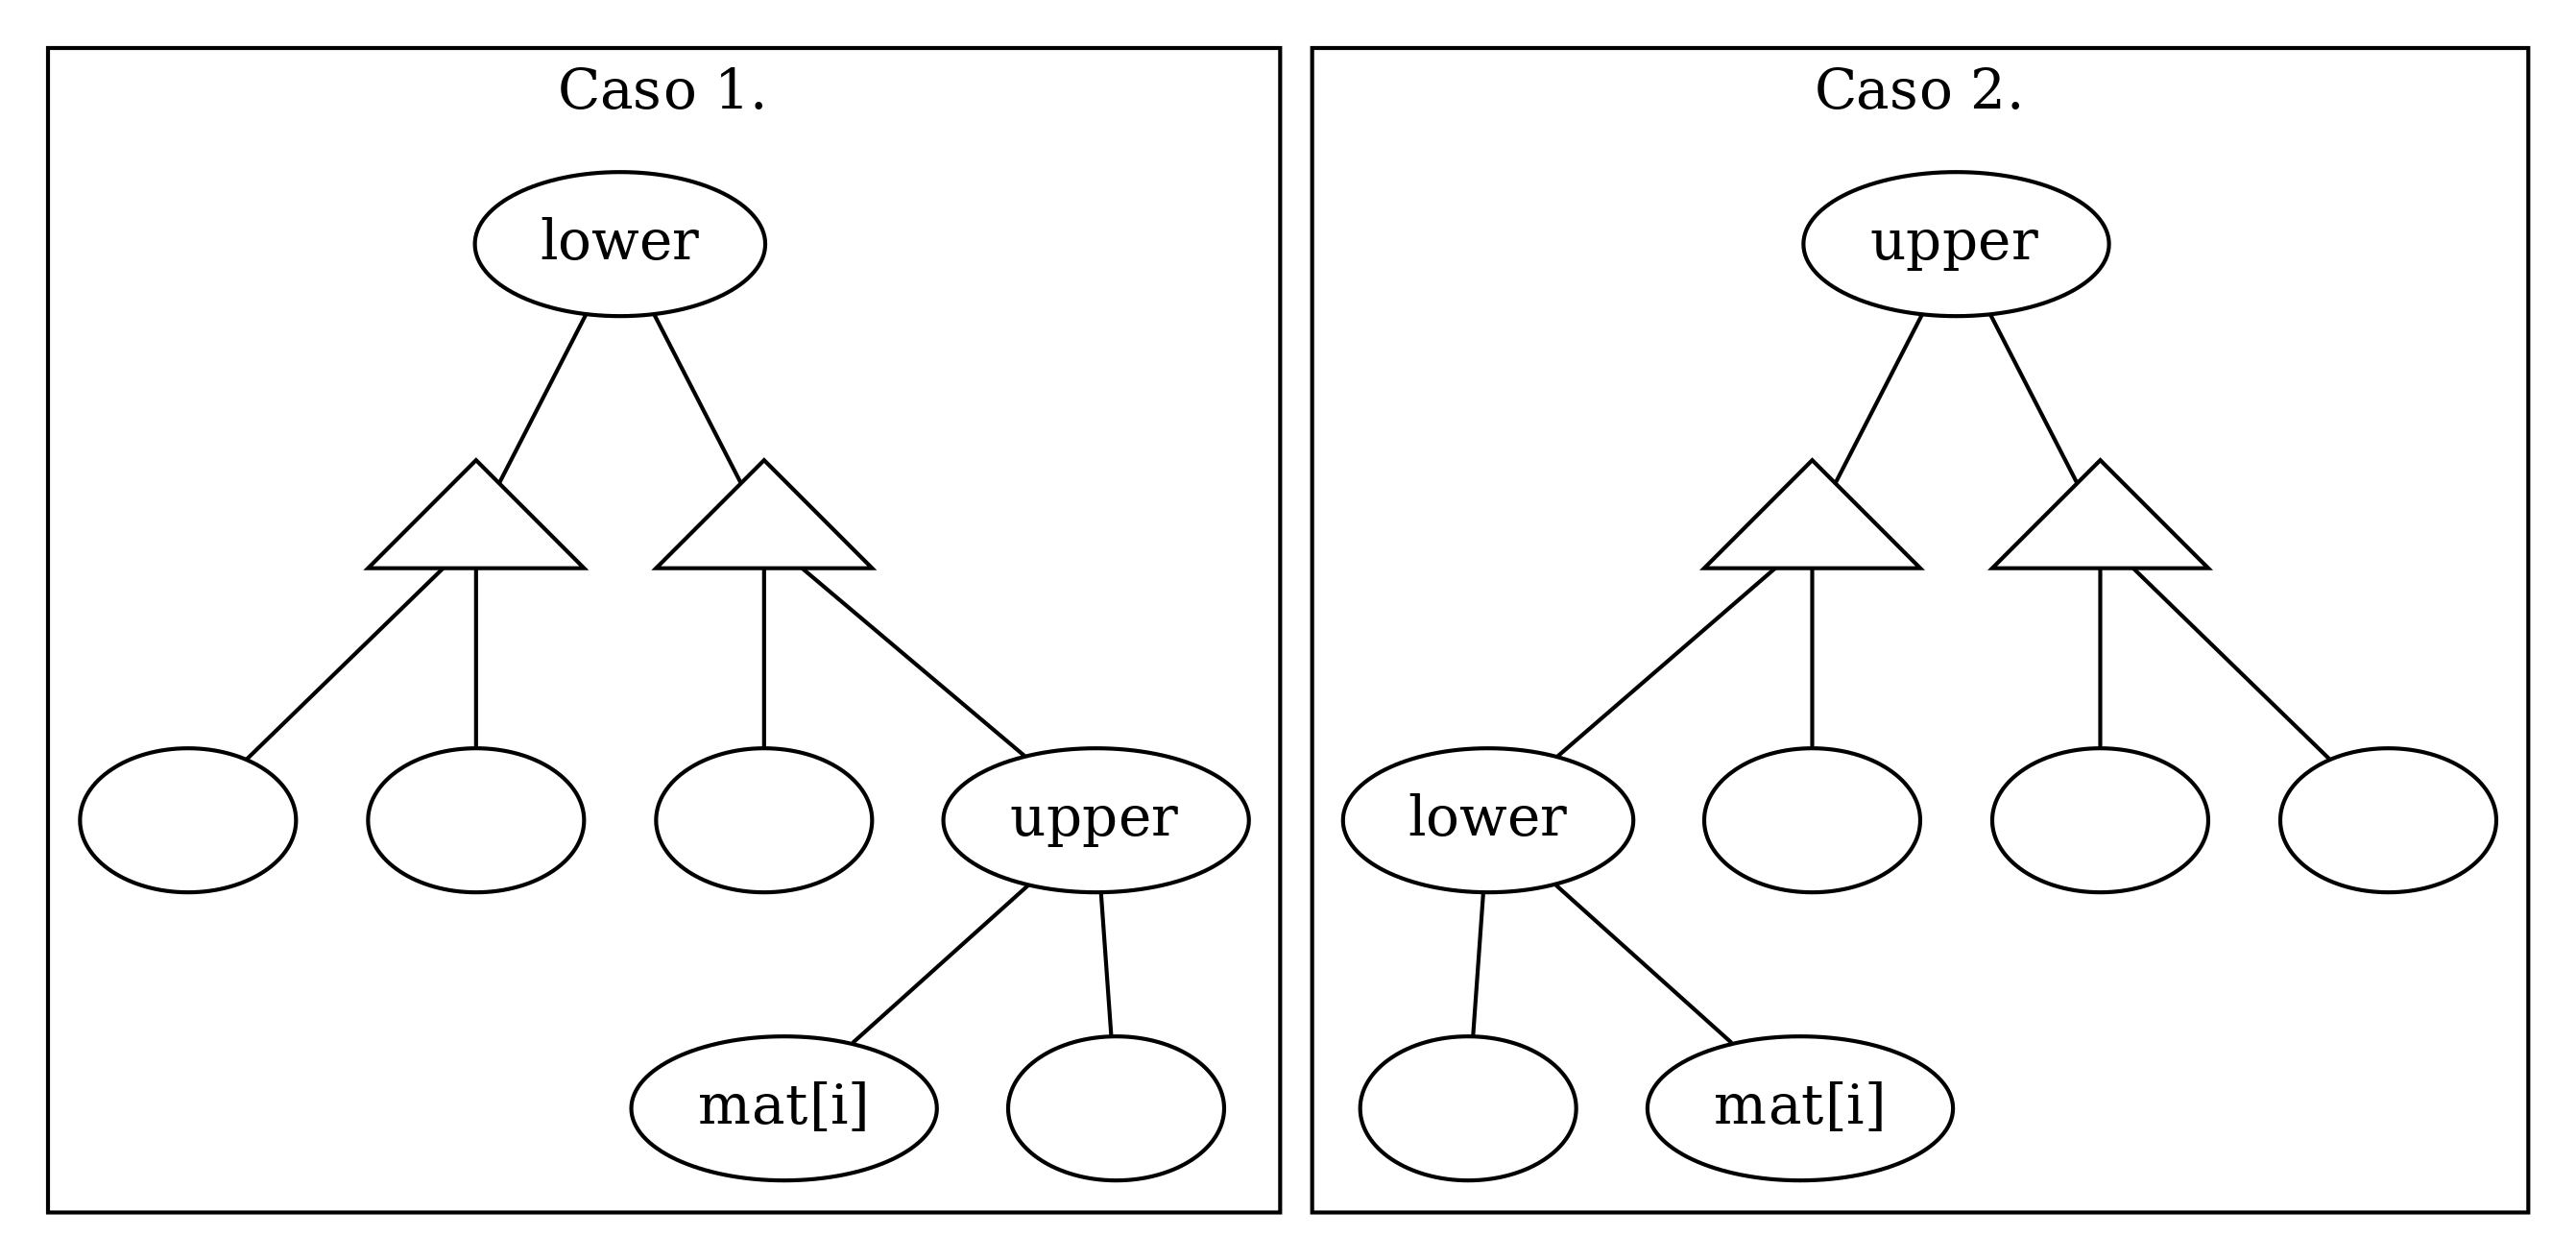
\includegraphics[width=0.7\linewidth]{lxu.png}

\begin{forest}
[$lower$, ellipse
	[$\cdots$, fit=band]
	[$\cdots$, edge=dashed
		[, phantom]
		[$upper$, ellipse, edge=dashed
			[{$mat[i]$}]
			[$\cdots$, edge=dashed]
		]
	]
]
\node at (current bounding box.south)    [below=1ex,draw,rectangle]{Caso 1};
\end{forest}
\hspace{1em}
\begin{forest}
[$upper$, ellipse
	[$\cdots$, edge=dashed
		[$lower$, ellipse, edge=dashed
			[$\cdots$, edge=dashed]
			[{$mat[i]$}]
		]
		[, phantom]
	]
	[$\cdots$, fit=band]
]
\node at (current bounding box.south)    [below=1ex,draw,rectangle]{Caso 2};
\end{forest}

\caption{Se $mat[i]$ será inserido entre duas matrículas na sequência, existem dois casos para a estrutura da ABB.}
\label{fig:lxu}
\end{figure}

Nesse passo temos duas configurações possíveis, como pode ser visto
na figura~\ref{fig:lxu}, portanto precisamos determinar quem está na subárvore
de quem (linha 14) para escolher a configuração correta: se $upper$ está na subárvore de $lower$ (caso 1) então $upper$ é pai de $mat[i]$ (linhas 15--17), caso contrário (caso 2) $lower$ é pai de $mat[i]$ (linhas 19--21). Ao final do algoritmo a
tabela $parent$ possui os tutores de cada aluno.

\subsubsection{Análise da complexidade}
As operações \textsc{Max}, \textsc{Min}, \textsc{Previous},
\textsc{Insert}($parent$) e \textsc{Insert}($level$), inserção em tabela
\textit{hash}, possuem complexidade O(1), enquanto a operação
\textsc{LowerBound} é O($\lg n$), em que $n$ é a quantidade de elementos na árvore. Como discutido na seção~\ref{sec:algo}
a operação \textsc{Insert}($order$), utilizando análise amortizada, possui
complexidade O($m \lg n$), para $m$ operações. Analogamente, por análise amortizada, a operação
\textsc{LookUp}, de uma tabela \textit{hash} com tratamento de colisão por
encademaneto, possui complexidade O(1). Com isso, os trechos 3--7, 8--11 e
12--21 possuem complexidade O(1), então o bloco entre 3--24 tem complexidade O(1). Concluímos,
portanto que a complexidade do algoritmo \textsc{Parents} é, pela aproximação de
Stirling:
\begin{align*}
  \sum_{i = 1}^{N}(\text{O}(\lg i) + \text{O}(1) + \text{O}(\lg i)) = \sum_{i = 1}^{N}(\text{O}(\lg i)) = \text{O}(\lg \prod_{i = 1}^{N} i) = \text{O}(\lg N!) \sim N \lg N
      % ~\text{O}(n \lg n)
\end{align*}